\section{State of the art}


%%%%%%%%%%%%%%%%%%%%%%%%%%%%%%%%%%%%%%%%%%%%%%%%%%%%%%%%%%%%%%%%%%%%%%%%%%%%%%%
\begin{frame}{The CAP theorem}{Consistency vs. Availability}

\begin{block}{Eric Brewer's theorem}
``A shared-state system can have \textbf{at most two} of the following properties at any given time:

\begin{itemize}
	\item \textbf{C}onsistency
	\item \textbf{A}vailability
	\item \textbf{P}artition tolerance''
\end{itemize}
\end{block}


\begin{center}
\Large 
Under network partitions, a distributed data store has to sacrifice either availability or consistency.
\end{center}
\vfill

\begin{itemize}
	\item \textbf{Consistency-first}: Abort incoming queries;
	\item \textbf{Availability-first}: Return possibly stale data.
\end{itemize}

\end{frame}

%%%%%%%%%%%%%%%%%%%%%%%%%%%%%%%%%%%%%%%%%%%%%%%%%%%%%%%%%%%%%%%%%%%%%%%%%%%%%%%
\begin{frame}{Consistency-first: the ACID model}{Consistency vs. Availability}

\textbf{Transaction}: unit of work within an ACID data store. 
%Comprises multiple operations.
%E.g. bank transfer.
%E.g. a bank transfer from A to B is a transaction involving two operations: withdraw money from A & credit B with the same money amount. 
\vfill

\begin{itemize}
	\item \textbf{\underline{A}tomicity}: Transactions either complete entirely or fail.

	No transaction ever seen as in-progress.

	\item \textbf{\underline{C}onsistency}: Transactions always generate a valid state.

	The database maintains its invariants across transactions.

	\item \textbf{\underline{I}solation}: Concurrent transactions are seen as sequential.

	Transactions are serializable, or sequentially consistent.

	\item \textbf{\underline{D}urability}: Committed transactions are never forgotten.
\end{itemize}
\vfill\centering

Reads are fast, writes are slow.

\vfill\raggedright

Example: relational databases.
\end{frame}

%%%%%%%%%%%%%%%%%%%%%%%%%%%%%%%%%%%%%%%%%%%%%%%%%%%%%%%%%%%%%%%%%%%%%%%%%%%%%%%
\begin{frame}[fragile]{Concurrent writes in ACID}{Consistency vs. Availability}


\begin{columns}
\column{.5\columnwidth}
	\begin{block}{}
		\begin{lstlisting}
transaction AcqDoses(y):
  x <- SELECT #vaccines;
  UPDATE #vaccines = (x + y);
		\end{lstlisting}
	\end{block}
	\vspace{5ex}

	Supports compound operations.
\column{.5\columnwidth}
\centering
\includegraphics[width=\columnwidth]{figures/conflict_acid.pdf}
\end{columns}

\end{frame}


%%%%%%%%%%%%%%%%%%%%%%%%%%%%%%%%%%%%%%%%%%%%%%%%%%%%%%%%%%%%%%%%%%%%%%%%%%%%%%%
\begin{frame}{Availability-first: the BASE model}{Consistency vs. Availability}


Some apps prefer availability, e.g. Amazon products' reviews.
\vfill 

The BASE model trades Consistency \& Isolation for Availability.


%Some applications do not care about strong consistency and prefer being highly available (e.g. Amazon's product reviews).

%In order to achieve higher availability, the BASE model relaxes consistency constraints of the ACID model: "eventual consistency".
\vfill

\begin{itemize}
	\item \textbf{\underline{B}asic \underline{A}vailability}: 
	The data store thrives to be available.

	\item \textbf{\underline{S}oft-state}: 
	Replicas can disagree on the valid state.

	\item \textbf{\underline{E}ventual consistency}: 
	In the absence of write queries, 
	the data store will eventually converge to a single valid state.
\end{itemize}
\vfill\centering

Writes are fast, reads are slow.

\vfill\raggedright

Examples: key-value \& object stores.

\end{frame}

%%%%%%%%%%%%%%%%%%%%%%%%%%%%%%%%%%%%%%%%%%%%%%%%%%%%%%%%%%%%%%%%%%%%%%%%%%%%%%%
\begin{frame}{Concurrent writes in BASE}{Consistency vs. Availability}

\begin{columns}
\column{.5\columnwidth}
	\begin{block}{Object}
		\begin{itemize}
			\item Unique key
			\item Arbitrary value 
			\item Metadata
		\end{itemize}
	\end{block}
	\vspace{5ex} 

	Conflict resolution = client's job!
	\vspace{5ex}

	No compound operations.
\column{.5\columnwidth}
	\centering
	\includegraphics[width=\columnwidth]{figures/conflict_base.pdf}
\end{columns}

% KV storage is another example, distinction is minor here

% Object = unique key, arbitrary value, metadata.

% Object storage only provides semantics to investigate causal order of queries *for individual objects*. No compound operations, no transactions.

% Much easier to distribute, and "scale-out".

% Write is fast, read is slow (gotta collect all object versions).

% \todo{vaccines example with BASE model}

\end{frame}

%%%%%%%%%%%%%%%%%%%%%%%%%%%%%%%%%%%%%%%%%%%%%%%%%%%%%%%%%%%%%%%%%%%%%%%%%%%%%%%
\begin{frame}{Strong Eventual Consistency w/ CRDTs}{Consistency vs. Availability}

\centering\small

\fullcite{defago_conflict-free_2011}

\vfill\raggedright\normalsize

\begin{block}{Strong Eventual Consistency (SEC)}
	\begin{itemize}
		\item CRDTs specify distributed operations
		\item Conflicts will be solved according to specification
		\item Proven \& bound eventual convergence
	\end{itemize}
\end{block}

\vfill\centering

\includegraphics[width=.5\columnwidth]{figures/crdt.pdf}

\end{frame}

%%%%%%%%%%%%%%%%%%%%%%%%%%%%%%%%%%%%%%%%%%%%%%%%%%%%%%%%%%%%%%%%%%%%%%%%%%%%%%%
\begin{frame}[fragile]{Concurrent writes with CRDTs}{Consistency vs. Availability}

\begin{columns}
\column{.5\columnwidth}
	\begin{block}{}
		\begin{lstlisting}
CRDT Counter(x0):
  history = {}
  op. incr(y):
    history U= {(UUID(), y)}
  op. decr(y):
    history U= {(UUID(), -y)}
  op. read():
    x = x0
    for (_, y) in history:
    	x += y
    return x
		\end{lstlisting}
	\end{block}
	\vspace{2ex}

	Operations commute?

	$\implies$ screw total order!
\column{.5\columnwidth}
	\centering
	\includegraphics[width=\columnwidth]{figures/conflict_crdt.pdf}
\end{columns}

\end{frame}


%%%%%%%%%%%%%%%%%%%%%%%%%%%%%%%%%%%%%%%%%%%%%%%%%%%%%%%%%%%%%%%%%%%%%%%%%%%%%%%
\begin{frame}{A complex CRDT: the DAG}{Consistency vs. Availability}

\centering
\only<1>{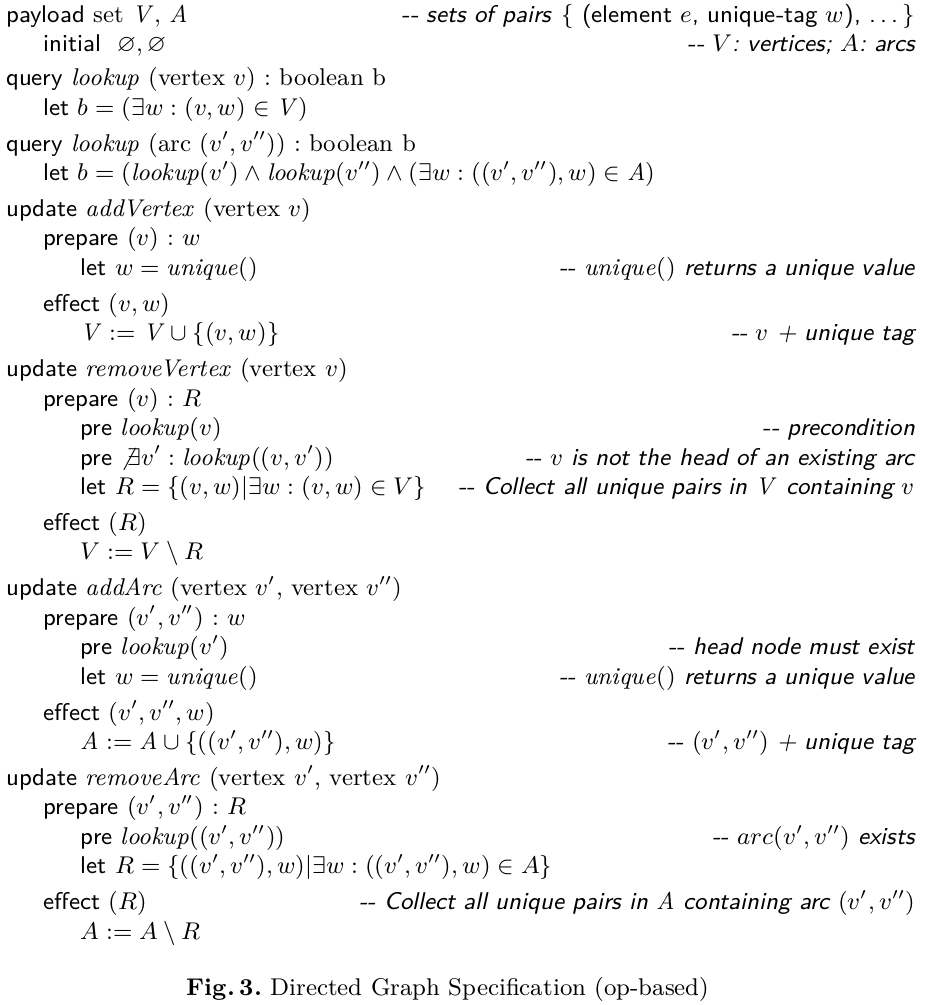
\includegraphics[height=\textheight]{figures/dag_crdt.png}}%
\only<2>{
	Just to say I swept a lot under the rug.
	\vfill

	For details, go read:

	\fullcite{defago_conflict-free_2011}
	\vfill

	For an implementation, check \textbf{AntidoteDB}.
}

\end{frame}

%%%%%%%%%%%%%%%%%%%%%%%%%%%%%%%%%%%%%%%%%%%%%%%%%%%%%%%%%%%%%%%%%%%%%%%%%%%%%%%
\begin{frame}{State of the practice}{Path dependency to the ``cloud''}

\begin{block}{The BASE model is fashionable because}
\centering 

``\emph{High-performance} object storage for \emph{AI analytics} with PBs of \emph{IoT data streams} at the \emph{edge}, using \emph{5G}.''
	% \begin{itemize}
	% 	\item Highest performance 
	% 	\item IoT data streams are inherently distributed
	% \end{itemize}
\end{block}

\vfill\centering

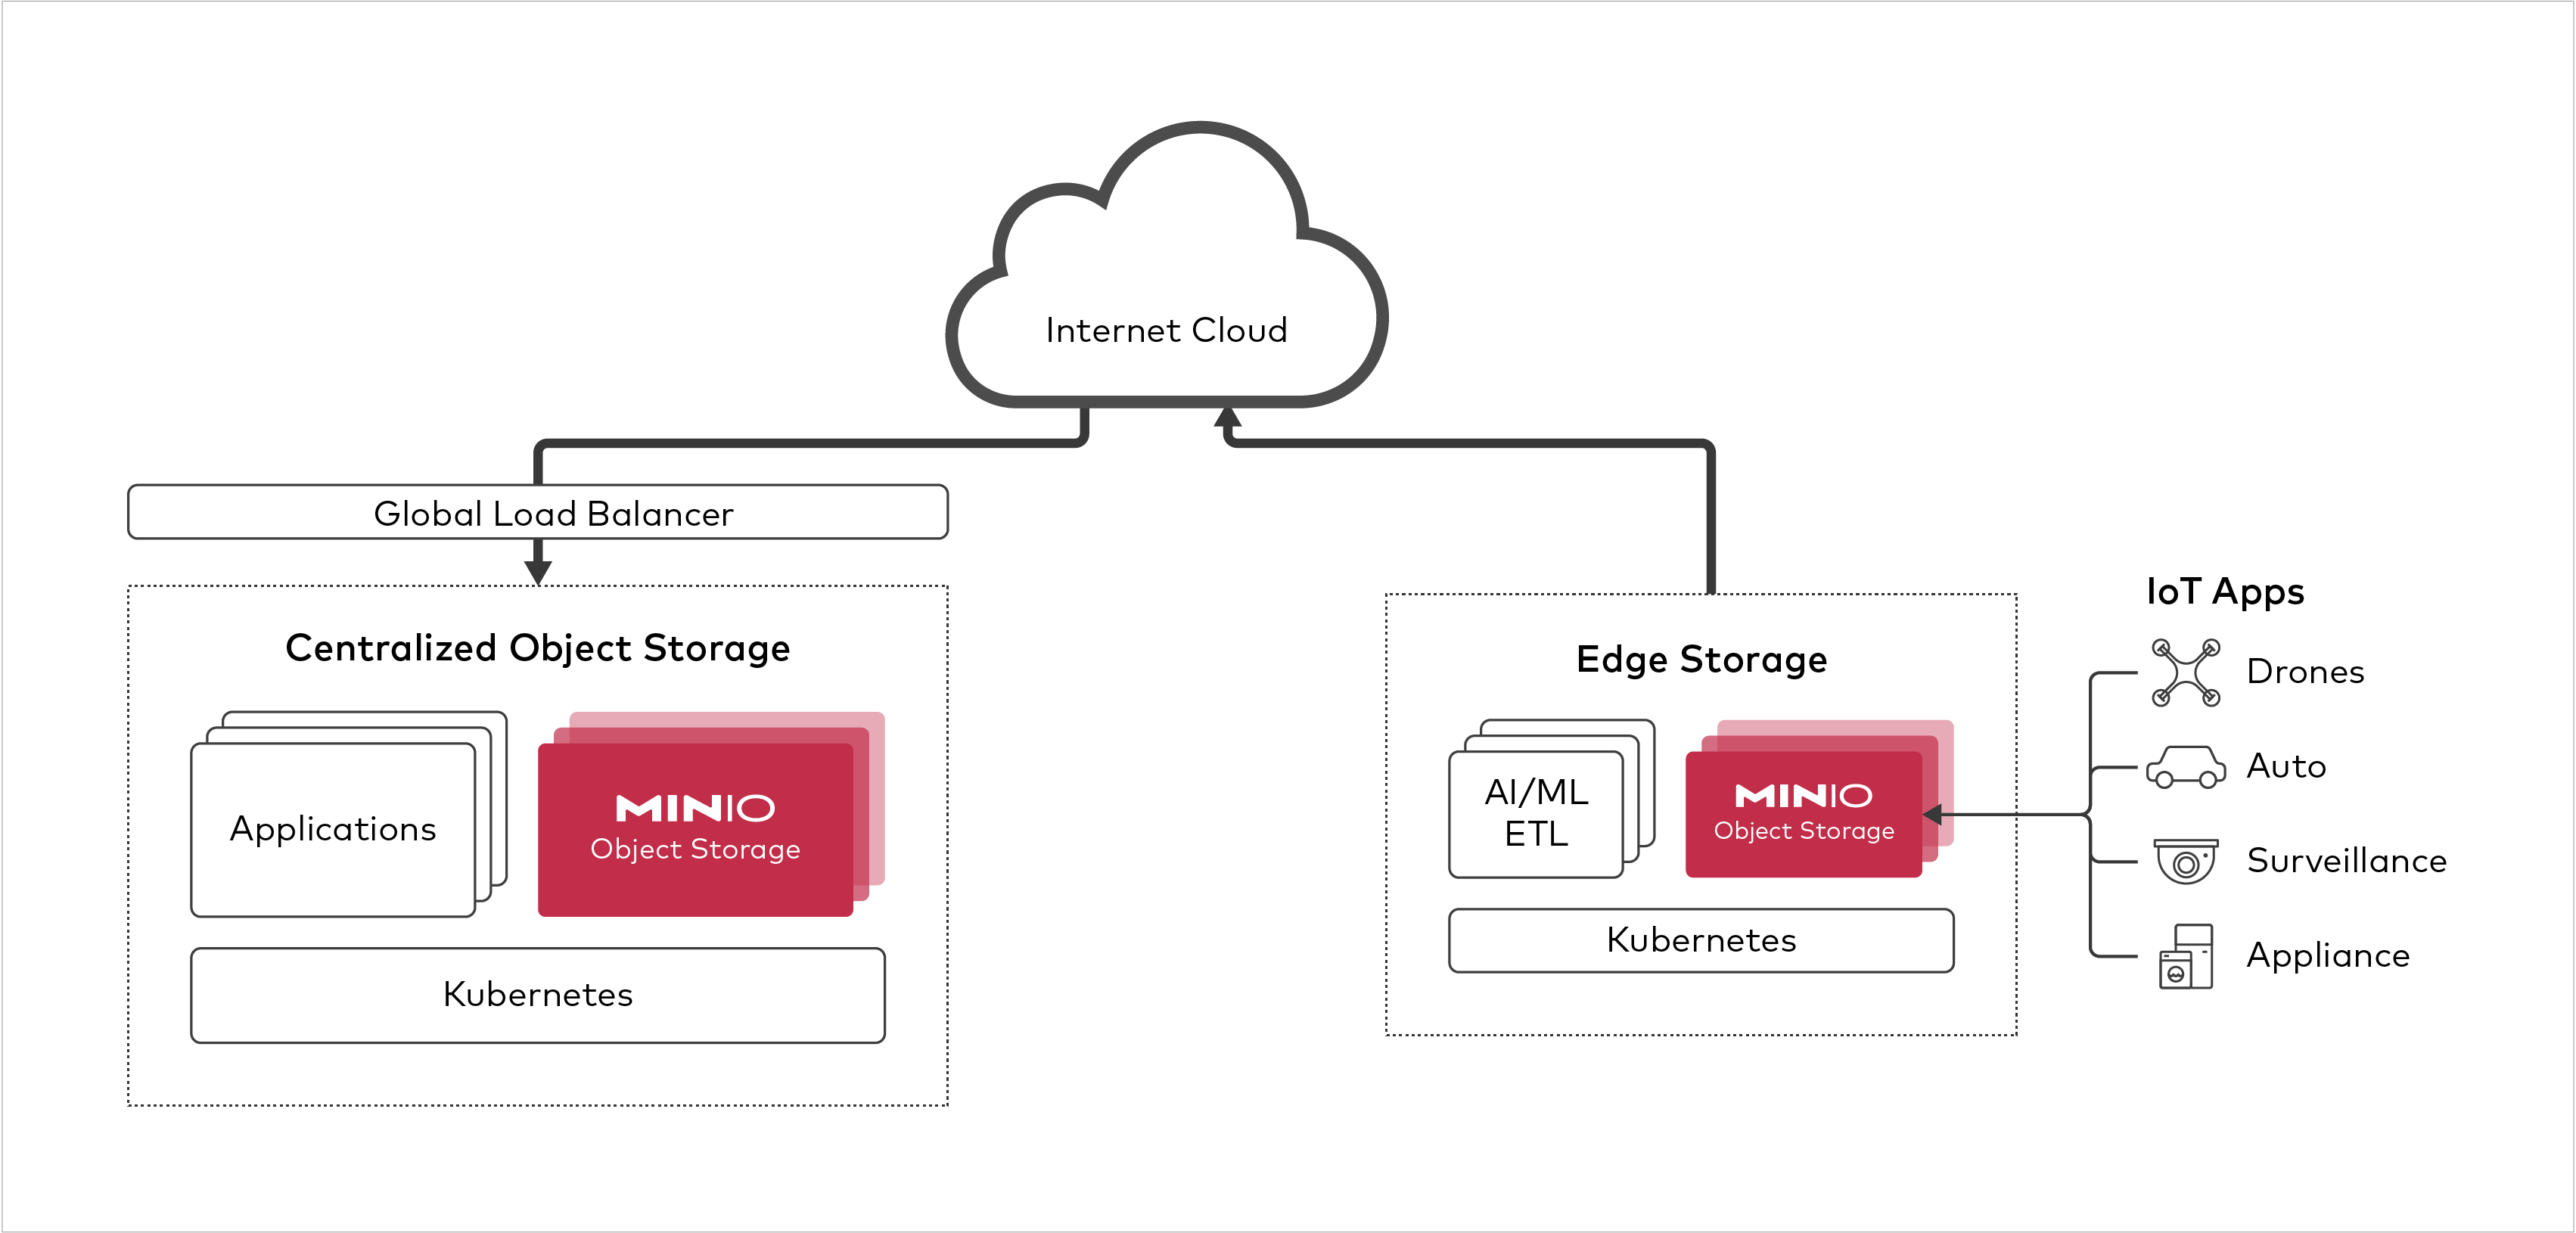
\includegraphics[width=.9\columnwidth]{figures/minio_edge.png}

\vfill\raggedright


%\begin{block}{}
\begin{itemize}
	\item Always backed by cloud: high performance network links.
	\item Edge nodes always seen as clients or data sources, not peers.
\end{itemize}
%\end{block}

% There is \textbf{always a central cloud cluster} in these use-cases.

% Hidden constraint: \textbf{high performance inter-node connectivity}.



\end{frame}



%%%%%%%%%%%%%%%%%%%%%%%%%%%%%%%%%%%%%%%%%%%%%%%%%%%%%%%%%%%%%%%%%%%%%%%%%%%%%%%
%%%%%%%%%%%%%%%%%%%%%%%%%%%%%%%%%%%%%%%%%%%%%%%%%%%%%%%%%%%%%%%%%%%%%%%%%%%%%%%
% \begin{frame}{A brief history of storage}

% We keep it short because we'll follow chronological order in the next section too.

% \end{frame}


% \begin{frame}{In the beginning, there were \emph{monoliths}}

% \includegraphics[width=.5\columnwidth]{figures/stonehenge.jpg}

% Web applications used to be monolithic:

% \begin{itemize}
% 	\item One or two servers;
% 	\item Availability was not an obsession;
% 	\item Latency was acceptable.
% \end{itemize}

% Relational databases were queens.

% \end{frame}


% \begin{frame}{Then came \emph{expectations}}
% Then, the whole world went online, and suddenly: expectations!

% \begin{itemize}
% 	\item ``Milliseconds matter.'' (Algolia slogan)
% 	\item Critical networked services (healthcare, logistics) need 100\% availability 
% \end{itemize}

% $\implies$ Microservices \& horizontal scalability.

% \todo{Develop on the `herd not sheep' paradigm a bit.}

% \end{frame}


% \begin{frame}{Distributing state/storage: the remaining unknown}

% The microservices orchestration game works well for \emph{stateless} services.

% However, any application requires \emph{state}, persistent data. 

% And this is tough. As we will now see.

% (Not that it's not well studied: distributed storage has always been fashionable.)
	
% \end{frame}